\documentclass[lecture_notes.tex]{subfiles}

\begin{document}

\notestitle{Session 3}{Exact Diagonalization in the Fermionic Basis}%
  {quantum\_interacting\_fermions.ipynb}{Session 1 (second quantization, the Hubbard model,
  mean-field theory); Session 2 (exact diagonalization, though we rebuild everything we need
  directly in the fermionic language here)}

\section*{Contents and goals}
Session 1 built the Hubbard model from second quantization and solved it at the mean-field level,
and it ended on a warning: mean-field theory can fail badly, even on the smallest possible
example, the Hubbard dimer at half filling. Session 2 picked up right at that failure point and
solved the resulting Heisenberg spin model exactly, with no product-state restriction at all, by
diagonalizing directly in the spin basis. In this session we go back one step further and
diagonalize the \emph{original} fermionic Hamiltonian exactly, working in the fermionic Fock space
itself rather than first mapping onto spins. This is not just a change of language: it lets us see
things a spin model simply cannot represent, charge physics, a real chemical potential, a genuine
insulator-versus-metal distinction, and, most strikingly, a completely numerically exact test of
Session 1's mean-field magnetization prediction. We will find that mean-field theory gets the
Hubbard chain's magnetization qualitatively wrong, not just quantitatively wrong, which is exactly
the kind of failure that motivates doing things exactly whenever we can afford to. We close by
watching spin and charge decouple from each other as the interaction grows, a genuinely many-body
effect called spin-charge separation. Session 5 will pick this exact fermionic program back up and
push it to far larger system sizes using tensor networks.

\section*{Learning outcomes}
By the end of this session, you should be able to:
\begin{itemize}[nosep]
  \item Diagonalize interacting fermionic Hamiltonians directly in Fock space and explain how the
    Hilbert-space dimension scales with system size and spin.
  \item Use ground-state degeneracy, a chemical-potential sweep, and the charging energy to
    identify a charge-density-wave transition and control the ground-state particle number.
  \item Test Session 1's mean-field magnetization prediction against the exact Hubbard result and
    explain the disagreement using Lieb's theorem.
  \item Diagnose spin-charge separation from static and dynamical correlators, and connect the
    strong-coupling limit to the Heisenberg model of Session 2.
\end{itemize}

\section{From spins back to fermions: the many-body Fock space}
Let us start by rebuilding the same many-body machinery we used for spins in Session 2, but now
directly in terms of fermionic creation and annihilation operators. Recall from Session 1 that a
single-particle Hamiltonian acting on $L$ orbitals is just an $L\times L$ matrix, and diagonalizing
it costs polynomial time. The moment we add any quartic (interaction) term, that is no longer true:
we have to diagonalize $\Ham$ in the full many-body Fock space, spanned by all the ways of
distributing electrons among the $L$ orbitals, and that space grows exponentially in $L$.

Let us count this explicitly, the same way the lecture does. Take two spinless sites, labeled $0$
and $1$. The many-body basis has exactly four states,
\begin{equation}
  \vac, \qquad \cre{0}\vac, \qquad \cre{1}\vac, \qquad \cre{0}\cre{1}\vac,
\end{equation}
the empty state, the two singly-occupied states, and the doubly-occupied state, so $\Ham$ is a
$4\times4$ matrix in this basis. Add a third site and the counting becomes $1 + 3 + 3 + 1 = 8$
states (one empty configuration, three with one electron, three with two electrons, one fully
filled), which is $2^3$. In general, for $L$ spinless orbitals the Fock space has dimension $2^L$:
every orbital is independently either empty or filled, so we get one binary choice per orbital.
This is worth contrasting with the single-particle sector alone, spanned by $\cre{i}\vac$ for
$i=1,\dots,L$, which only has dimension $L$: restricting to one electron is precisely what makes
single-particle physics polynomially cheap, and dropping that restriction is precisely what makes
many-body physics exponentially expensive.

\begin{figure}[H]
  \centering
  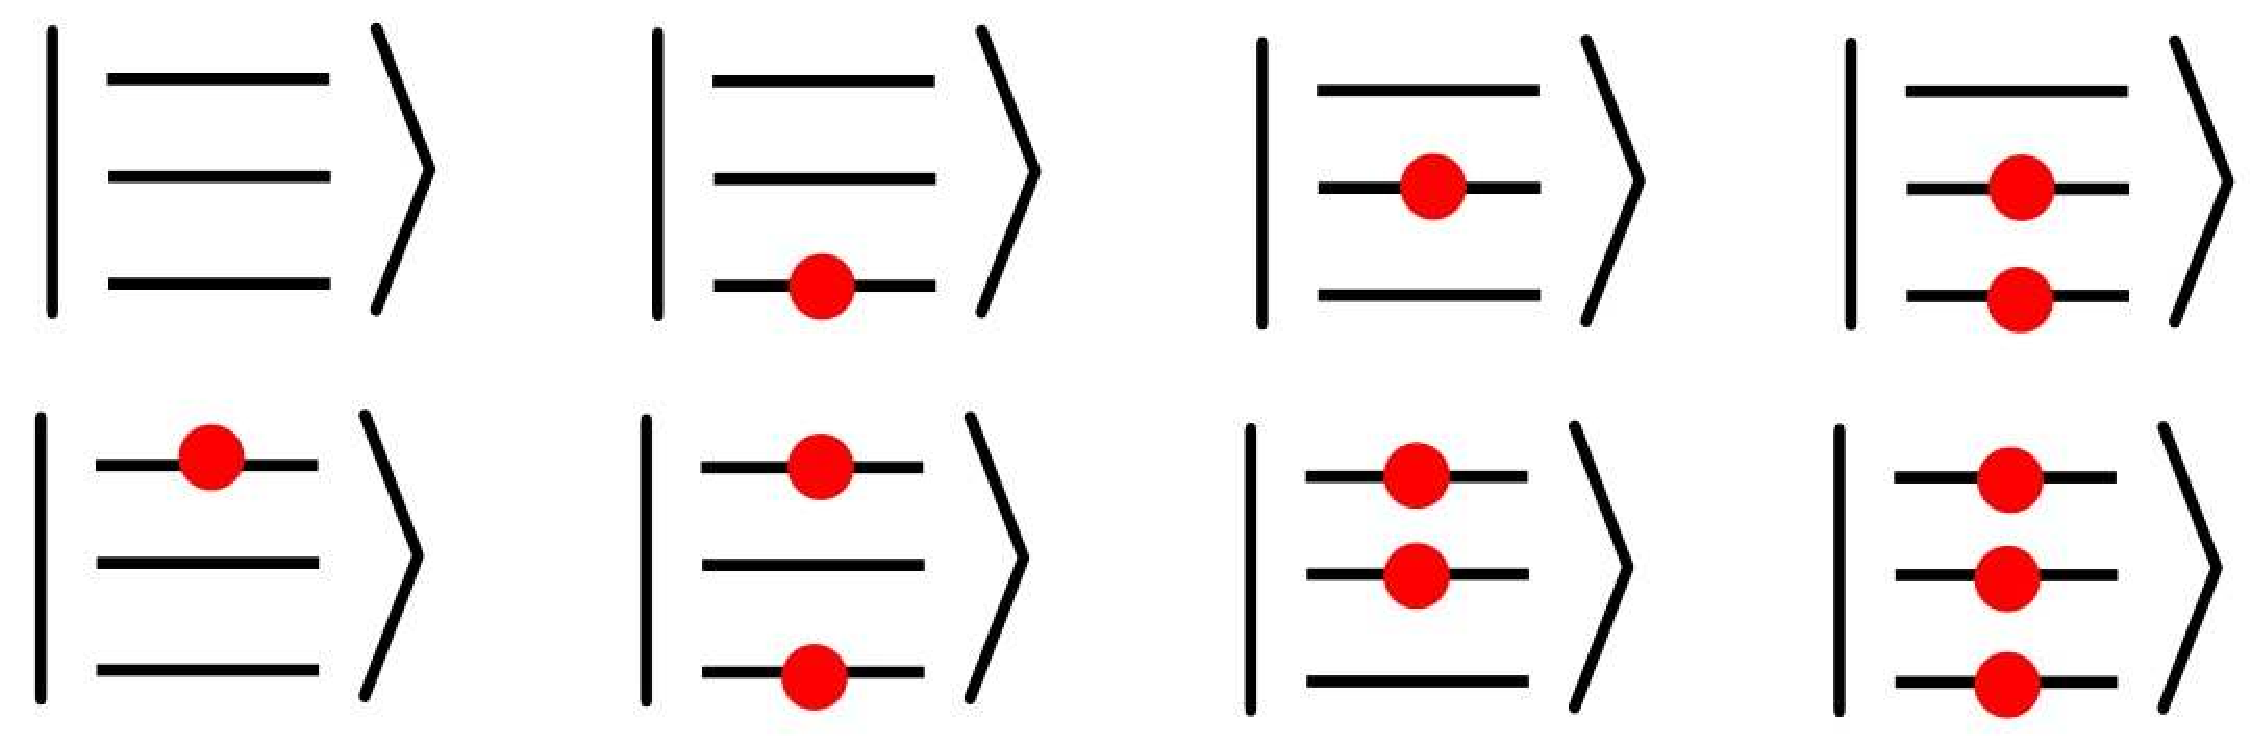
\includegraphics[width=0.85\textwidth]{figures/many_body_fermions/fock_space_trimer_basis.pdf}
  \caption{The complete many-body basis of three spinless orbitals, drawn as three levels per
    state with a dot on every occupied one. Reading across, there is one empty configuration,
    three with a single electron, three with two electrons and one completely filled state, for
    $1+3+3+1 = 8 = 2^3$ basis states in total. Every additional orbital doubles this count,
    because each orbital is independently either empty or filled, and that doubling is exactly
    the exponential wall that separates many-body from single-particle physics.}
  \label{fig:fock-basis}
\end{figure}

If the fermions carry spin, each site has \emph{four} local states, $\ket{0}$, $\ket{\up}$,
$\ket{\dn}$, $\ket{\up\dn}$, exactly as in Session 1. Equivalently, we can think of a spinful chain
as $2L$ independent spinless orbitals (spin becomes just another orbital index), so the Fock space
has dimension $2^{2L} = 4^L$: twice the exponent of the spinless case, since every site now
contributes two binary choices instead of one. It is worth pausing on how this lines up with the
spin chains of Session 2: an $L$-site spin-$\tfrac12$ chain also has a $2^L$-dimensional Hilbert
space, exactly matching the spinless-fermion count. This is not a coincidence: a rigorous mapping
(Jordan--Wigner, which we will meet properly in Session 5) sends spinless fermions to spin-$\tfrac12$
degrees of freedom one-for-one. For now, the practical upshot is simply this:
\begin{itemize}[nosep]
  \item solving an interacting \textbf{spinless} fermionic chain costs exactly as much as
    solving a quantum \textbf{spin} chain of the same length, $\sim 2^L$;
  \item solving an interacting \textbf{spinful} fermionic chain, like the Hubbard model, costs the
    square of that, $\sim 4^L$, so at fixed computational budget we can only reach about half the
    system size.
\end{itemize}
Just as in Session 2, once we have $\Ham$ written as an explicit $2^L\times2^L$ (or $4^L\times4^L$)
matrix in this Fock basis, the ground state is simply its lowest eigenvector, a set of $2^L$ (or
$4^L$) complex coefficients multiplying each basis configuration, and any expectation value we
want, $\expval{n_i}$, $\expval{S_i^z}$, correlators, spectra, follows by ordinary linear algebra on
that eigenvector. No approximation, no product-state restriction: this is the entire promise of
exact diagonalization, now made good on directly in the fermionic language.

\begin{notebook}
Sections ``Creating a fermion\_chain object,'' ``Creating a Hamiltonian,'' ``Computing the ground
state energy,'' and ``Computing expectation values.'' Build a small fermionic chain object, write
down a many-body Hamiltonian directly in terms of the fermionic operators, and extract its ground
state energy and a couple of expectation values. This is the fermionic analogue of what you did
with spin operators in Session 2, and it is worth comparing the two interfaces side by side.
\end{notebook}

\section{The spinless-fermion model: a charge-density-wave transition, computed exactly}
\label{sec:cdwexact}
Let us put this machinery to work on the simplest interacting model we have: the spinless
nearest-neighbor chain from Session 1,
\begin{equation}
  \Ham_{\mathrm{CDW}} = -t\sum_i\left(\cre{i}\ann{i+1} + \mathrm{h.c.}\right)
    + V\sum_i \left(n_i - \tfrac12\right)\left(n_{i+1} - \tfrac12\right), \qquad n_i \equiv
    \cre{i}\ann{i}.
  \label{eq:cdw3}
\end{equation}
This is exactly Session 1's $\Ham_{\mathrm{CDW}}$, just with $n_i \to n_i - \tfrac12$ inside the
interaction, a purely bookkeeping shift: expanding it out just adds a constant plus an automatic
chemical potential of $-V/2$ per site, tuned so that the model sits exactly at half filling without
us needing to add and adjust a separate $\mu$ by hand.

Two limits of Eq.~\eqref{eq:cdw3} are easy to solve outright. At $V=0$ we just have the free
tight-binding chain of Session 1: a single cosine band, filled up to the Fermi points, a metal with
a unique, non-degenerate ground state. At $V\to\infty$ we can drop the hopping altogether, and the
interaction alone is minimized by the classical alternating pattern $1,0,1,0,\dots$: exactly one
electron every other site. There are exactly \emph{two} such states, related by shifting the pattern
by one site, and they are degenerate: this is the charge-density wave, and its defining signature
is that the ground state is twofold degenerate, in sharp contrast with the unique metallic ground
state at $V=0$.

\begin{figure}[H]
  \centering
  \begin{subfigure}[c]{0.41\textwidth}
    \centering
    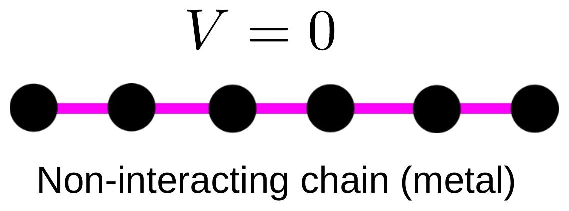
\includegraphics[width=\linewidth]{figures/many_body_fermions/cdw_schematic_metal.pdf}
    \caption{Uniform density}
  \end{subfigure}\hfill
  \begin{subfigure}[c]{0.49\textwidth}
    \centering
    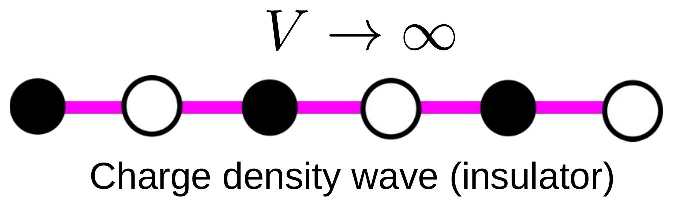
\includegraphics[width=\linewidth]{figures/many_body_fermions/cdw_schematic_insulator.pdf}
    \caption{Alternating occupation}
  \end{subfigure}
  \caption{The two solvable limits of Eq.~\eqref{eq:cdw3}, with filled circles marking occupied
    sites and open circles empty ones. (a) At $V=0$ the chain is a free tight-binding metal at
    half filling, with the same average density on every site and a unique ground state. (b) As
    $V\to\infty$ the hopping becomes irrelevant and the interaction alone selects the alternating
    $1,0,1,0,\dots$ pattern. Shifting that pattern by one site produces a second state of
    identical energy, and this twofold degeneracy is the defining signature of the
    charge-density wave.}
  \label{fig:cdw-limits}
\end{figure}

This is precisely what exact diagonalization lets us watch happen on a finite chain. Diagonalize
Eq.~\eqref{eq:cdw3} at fixed $L$ and plot the low-lying eigenvalues, measured relative to the
ground state, as a function of $V$. At small $V$ we see a unique ground state followed by a small
gap to a dense set of excited states: this gap is a finite-size artifact, roughly the level
spacing $\sim t/L$ of the underlying free-fermion band, and it visibly shrinks as we go from
$L=12$ to $L=14$, exactly as we would expect if it is destined to close in the thermodynamic limit
and leave behind a continuum. As $V$ grows, one particular excited state peels away from that
continuum and drops steadily toward the ground state, becoming exactly degenerate with it as
$V\to\infty$: this is the CDW partner state, and unlike the metallic gap, this near-degeneracy
does \emph{not} close by adding more excited states underneath it; instead a genuinely large gap
opens above the (now twofold) ground state, growing asymptotically as $\Delta \sim V$. That linear
growth has a simple interpretation: at large $V$, the cheapest way to excite the system is to
introduce a single domain wall into the alternating pattern, a local defect where the charge order
runs into itself, and each domain wall costs an energy of order $V$ regardless of the size of the
system, exactly the extensive, size-independent gap we see numerically.

It is worth comparing this directly with Session 1's mean-field treatment of the very same model.
There, the self-consistent gap also opened continuously as $V$ increased and also grew linearly at
large $V$, and here exact diagonalization confirms both of those features quantitatively. This is
not an accident: the CDW breaks a \emph{discrete} symmetry (translation by one site, a $\mathbb Z_2$
symmetry), and discrete symmetry breaking of this kind is allowed even in a one-dimensional quantum
system at zero temperature. Keep this in mind, because in Section~\ref{sec:hubbardmag} we will meet
a case where mean-field theory tries to break a \emph{continuous} symmetry, and there the story
changes completely.

\begin{notebook}
Sections ``Many-body energies of an interacting fermionic model'' and ``Towards
interaction-induced symmetry breaking.'' Plot the low-lying many-body spectrum of the spinless
chain as a function of $V$ for two system sizes, and identify by eye where the first excited state
collapses onto the ground state, this is the CDW transition. Then look at how the large-$V$ gap
scales with $V$ and check the linear behavior we derived above.
\end{notebook}

\section{Chemical potential, conserved quantum numbers, and the charging energy}
So far we have kept the electron number fixed at half filling. Let us now add a chemical potential
explicitly,
\begin{equation}
  \Ham(\mu) = \Ham_{\mathrm{CDW}} - \mu \sum_i n_i \equiv \Ham_{\mathrm{CDW}} - \mu N,
  \label{eq:muterm}
\end{equation}
where $N = \sum_i n_i$ is the total particle number operator. The key structural fact here is that
$[\Ham_{\mathrm{CDW}}, N] = 0$: hopping moves an electron from one site to another without changing
how many there are in total, and the interaction only counts electrons, so it commutes with $N$
trivially too. Since $\Ham_{\mathrm{CDW}}$ and $N$ commute, they share a common eigenbasis, which
means adding the $-\mu N$ term does not change a single eigenvector of $\Ham_{\mathrm{CDW}}$: it
only shifts each eigenenergy by $-\mu N$, where $N$ is that eigenstate's own, fixed particle
number. Concretely, this means every eigenvalue of $\Ham(\mu)$ traces out a straight line as a
function of $\mu$, with slope $-N$ set entirely by that state's particle number relative to the
ground state's.

This has an immediate and useful consequence: because different excited states carry different
particle numbers, they have different slopes, and as we sweep $\mu$ these lines cross. Right at a
crossing, the identity of the \emph{ground state} itself changes: below the crossing the
lowest-energy state has $N$ electrons, above it the lowest-energy state has $N\pm1$. In other
words, $\mu$ is a knob that directly controls the electron number of the ground state, exactly as
a gate voltage does in a real quantum dot or nanostructure.

Let us make this quantitative. Define $E(N)$ as the lowest eigenvalue of $\Ham_{\mathrm{CDW}}$
restricted to the $N$-particle sector. The state with $N$ particles is the ground state of
$\Ham(\mu)$ precisely when $E(N) - \mu N$ is lower than $E(N\pm1) - \mu(N\pm1)$, which rearranges
into a window,
\begin{equation}
  E(N) - E(N-1) \;<\; \mu \;<\; E(N+1) - E(N).
  \label{eq:addwindow}
\end{equation}
The width of this stability window is exactly the \textbf{charging energy},
\begin{equation}
  U_c(N) \equiv \big[E(N+1) - E(N)\big] - \big[E(N) - E(N-1)\big],
  \label{eq:charging}
\end{equation}
the discrete second derivative of the ground-state energy with respect to particle number. It
measures how much harder it gets to add one more electron than it was to add the previous one, and
it is exactly the quantity that produces the flat plateaus you see when you plot the ground-state
occupation $\expval{N}$ against $\mu$: on a plateau, $\mu$ can move freely without changing $N$,
because it has not yet exceeded the addition energy in Eq.~\eqref{eq:addwindow}. As $V$ grows, the
interaction makes it costlier to double up charge on already-crowded sites, $U_c$ grows with it,
and the plateaus in the $\expval{N}$-versus-$\mu$ curve widen accordingly, exactly what the
notebook shows you when you compare a weakly and a strongly interacting chain.

\begin{notebook}
Sections ``Energies of an interacting fermionic model as a function of the chemical potential,''
``Quantum numbers in the interacting fermionic model,'' ``Level crossings in the interacting
fermionic model,'' and ``Electronic density as a function of the chemical potential.'' Track the
particle number of each many-body eigenstate as $\mu$ is swept, watch the ground state switch
particle number at level crossings, and confirm that the width of each occupation plateau grows
with the interaction strength, exactly the charging-energy statement of
Eq.~\eqref{eq:charging}.
\end{notebook}

\section{The exact Hubbard magnetization: mean-field theory fails again}
\label{sec:hubbardmag}
Now let us bring spin back and repeat this exercise for the Hubbard chain,
\begin{equation}
  \Ham_{\mathrm{Hub}} = -t\sum_{i,\sigma}\left(\cre{i\sigma}\ann{i+1\sigma} + \mathrm{h.c.}\right)
    + U\sum_i \left(n_{i\up} - \tfrac12\right)\left(n_{i\dn} - \tfrac12\right),
  \label{eq:hub3}
\end{equation}
which, just as in Eq.~\eqref{eq:cdw3}, differs from Session 1's Hubbard Hamiltonian only by the
same bookkeeping shift, an automatic chemical potential that pins us at half filling.

Here is the punchline, and it is worth sitting with: if we diagonalize $\Ham_{\mathrm{Hub}}$
exactly and compute the local magnetization $m_i \equiv \expval{n_{i\up}} - \expval{n_{i\dn}}$ site
by site, we find $m_i = 0$ \emph{identically}, on every site, for every $U$, no matter how strong
the interaction is. This flatly contradicts what Session 1's mean-field theory told us to expect:
there, the self-consistency loop converges, for any $U>0$ on a bipartite half-filled chain, to a
finite staggered moment, $m_i = (-1)^i m$ with $m$ growing toward saturation as $U\to\infty$. Exact
diagonalization and mean-field theory are not just quantitatively different here, they disagree
about whether the ground state is magnetic at all.

This is not a numerical fluke; it follows from an exact symmetry argument. The Hamiltonian
Eq.~\eqref{eq:hub3} is invariant under any global spin rotation, so it commutes with the total spin
operators, $[\Ham_{\mathrm{Hub}}, \vb S^2] = [\Ham_{\mathrm{Hub}}, S_z^{\mathrm{tot}}] = 0$, and its
eigenstates can be labeled by a definite total spin $S$. \textbf{Lieb's theorem}
pins this down completely for the repulsive Hubbard model on any bipartite lattice at half filling:
the ground state is unique and has total spin $S = \tfrac12|N_A - N_B|$, where $N_A, N_B$ are the
sizes of the two sublattices. On our chain the sublattices are equal in size, so $S=0$ exactly, a
spin singlet, for every $U$ and every chain length. A rotationally invariant, unique, total-spin-zero
state simply cannot have a nonzero expectation value of $S_i^z$ on any individual site, since a spin
rotation would map it to an equally valid ground state with the opposite sign of $m_i$, and
uniqueness forbids two different ground states. Mean-field theory, by construction, searches only
over single Slater determinants, and a Slater determinant with staggered spin \emph{explicitly}
breaks spin-rotation symmetry from the very first guess: it can never represent a rotationally
invariant, entangled singlet, exactly the same structural failure we met with the Hubbard dimer in
Session 1.

\paragraph{Turning on an explicit symmetry-breaking field.} We can watch this failure mode directly
by interpolating between the exact model and the mean-field ansatz. Add an explicit staggered
field,
\begin{equation}
  \Ham(h) = \Ham_{\mathrm{Hub}} + h\sum_i (-1)^i \left(n_{i\up} - n_{i\dn}\right),
  \label{eq:stagger}
\end{equation}
which is precisely the single-particle term that mean-field theory would have generated on its own
had it found a self-consistent staggered solution (compare Session 1's $\HMF$). At $h=0$ we recover
the exact result, $m=0$. As $h$ increases from zero, $m(h)$ grows \emph{continuously} rather than
jumping to a finite value: quantum fluctuations, encoded in the entangled singlet ground state, are
actively fighting the ordering field, and only once $h$ is large enough to overwhelm those
fluctuations does $m(h)$ approach the mean-field saturation value. This is exactly the standard
diagnostic for spontaneous symmetry breaking: the true order parameter is defined as $m \equiv
\lim_{h\to0^+}\lim_{L\to\infty} m(h,L)$, and the order of these two limits matters enormously. At
any finite $L$, symmetry forces $m(h{=}0,L)=0$ exactly, so we must send $L\to\infty$ \emph{first}.
Even having done that, for the one-dimensional Heisenberg antiferromagnet that this model reduces
to at large $U$ (Section~\ref{sec:heisrecover}), this limit still gives zero: one dimensional
quantum antiferromagnets do not sustain true long-range magnetic order, only quasi-long-range,
power-law spin correlations, which is exactly the gaplessness we will meet again in
Section~\ref{sec:spincharge}. This is the deep reason mean-field theory fails so badly here: it is
not just missing quantitative corrections, it is predicting an ordered phase that, in one
dimension, does not exist.

\begin{table}[H]
\centering
\small
\begin{tabular}{@{}P{3.3cm}P{4.3cm}P{4.3cm}@{}}
\toprule
 & \textbf{CDW (Section~\ref{sec:cdwexact})} & \textbf{Hubbard magnetism (this section)} \\
\midrule
Symmetry broken & discrete, $\mathbb Z_2$ (one-site translation) & continuous, SU(2) (spin
rotation) \\
Mean-field prediction & finite $\delta n$, growing continuously with $V$ & finite staggered $m$,
growing continuously with $U$ \\
Exact 1D result & agrees qualitatively: order onset, gap $\sim V$ & disagrees: $m=0$ identically,
unique spin singlet \\
\bottomrule
\end{tabular}
\caption{The two symmetry-breaking scenarios met so far, contrasted: which symmetry is broken,
what mean-field theory predicts, and whether the exact one-dimensional result agrees.}
\label{tab:cdwvshubbard}
\end{table}

Table~\ref{tab:cdwvshubbard} lines up the two symmetry-breaking scenarios met so far side by
side: mean-field theory gets the discrete CDW transition qualitatively right, but gets the
continuous Hubbard magnetization badly wrong.

\begin{notebook}
Sections ``Magnetization of an interacting Hubbard model'' and ``Magnetization of a Hubbard model
with stagger magnetization.'' First confirm $m_i=0$ at every site of the exact Hubbard ground
state, however large $U$ is. Then switch on the staggered field of Eq.~\eqref{eq:stagger} and watch
$m$ grow smoothly from zero, and check how the field strength needed to saturate $m$ changes as you
increase $U$.
\end{notebook}

\section{Recovering the Heisenberg model: an exact worked example}
\label{sec:heisrecover}
Let us now directly verify, by exact diagonalization, the superexchange result $J \sim t^2/U$ that
Session 1 derived by degenerate perturbation theory. Take the Hubbard dimer, $L=2$, at half
filling, and work in the sector with zero total $S_z$, spanned by the four states
\begin{equation}
  \ket{1} = \cre{0\up}\cre{1\dn}\vac, \quad
  \ket{2} = \cre{0\dn}\cre{1\up}\vac, \quad
  \ket{3} = \cre{0\up}\cre{0\dn}\vac, \quad
  \ket{4} = \cre{1\up}\cre{1\dn}\vac,
\end{equation}
the same singly- and doubly-occupied configurations we met in Session 1. Hopping connects a singly
occupied state to a doubly occupied one but never $\ket{1}$ directly to $\ket{2}$, or $\ket{3}$
directly to $\ket{4}$, so in this basis $\Ham_{\mathrm{Hub}}$ (up to the constant $U/2$ shift from
Eq.~\eqref{eq:hub3}: the singly-occupied states sit at $-U/2$ and the doubly-occupied ones at
$+U/2$, so adding $U/2$ uniformly reproduces the diagonal below) is
\begin{equation}
  \Ham_{\mathrm{Hub}} \;\longrightarrow\;
  \begin{pmatrix} 0 & 0 & -t & t \\ 0 & 0 & t & -t \\ -t & t & U & 0 \\ t & -t & 0 & U\end{pmatrix}
  \quad\text{in the basis } \{\ket1,\ket2,\ket3,\ket4\}.
\end{equation}
This block diagonalizes cleanly if we pass to symmetric and antisymmetric combinations,
$\ket{a}=\tfrac1{\sqrt2}(\ket1+\ket2)$ (the $S_z=0$ member of the triplet), $\ket{b}=
\tfrac1{\sqrt2}(\ket1-\ket2)$ (the singlet), and likewise $\ket{c}=\tfrac1{\sqrt2}(\ket3+\ket4)$,
$\ket{d}=\tfrac1{\sqrt2}(\ket3-\ket4)$ for the doubly-occupied states. A short calculation shows
$\ket{a}$ and $\ket{c}$ are already exact eigenstates,
\begin{equation}
  \Ham_{\mathrm{Hub}}\ket{a} = 0\cdot\ket{a}, \qquad \Ham_{\mathrm{Hub}}\ket{c} = U\ket{c},
\end{equation}
while $\ket{b}$ and $\ket{d}$ mix into a genuine $2\times2$ block,
\begin{equation}
  \Ham_{\mathrm{Hub}}\big|_{\{b,d\}} = \begin{pmatrix} 0 & -2t \\ -2t & U\end{pmatrix}
  \;\Longrightarrow\;
  E_\pm = \frac{U \pm \sqrt{U^2 + 16t^2}}2.
\end{equation}
The lower eigenvalue, $E_-$, is the exact ground state, and comparing it against the exactly
degenerate $S_z=\pm1$ states $\ket{\up\up}$, $\ket{\dn\dn}$ (both sitting at energy $0$, just like
$\ket a$, since Pauli exclusion blocks all hopping for parallel spins), we see immediately that the
full ground state \emph{is} the total spin singlet ($S=0$), sitting strictly below the $S=1$
triplet at energy $0$, exactly as Lieb's theorem guaranteed in Section~\ref{sec:hubbardmag}. The
exact singlet-triplet gap is therefore
\begin{equation}
  \Delta_{\mathrm{s-t}} = 0 - E_- = \frac{\sqrt{U^2+16t^2} - U}{2}
  \;\xrightarrow[U\gg t]{}\; \frac{4t^2}{U},
  \label{eq:exactgap}
\end{equation}
which reproduces, from a completely independent, exact calculation, not just the $t^2/U$ scaling
but the exact same numerical prefactor that Session 1 obtained perturbatively for the effective
coupling $J=4t^2/U$ of $\Ham_{\mathrm{eff}} = J\,\vb S_1\cdot\vb S_2$: expanding
Eq.~\eqref{eq:exactgap} to leading order in $t/U$ gives $\Delta_{\mathrm{s-t}}\to4t^2/U$, digit for
digit. This is a genuinely satisfying check: two completely different techniques, one perturbative
and spin-only, one exact and fermionic, land on exactly the same physics, not just the same scaling.

\paragraph{Excitations as magnons.} We can probe the excited states further, exactly as in Session
2, by adding a Zeeman field $-h\,S_z^{\mathrm{tot}}$. Since $[\Ham_{\mathrm{Hub}}, S_z^{\mathrm
tot}]=0$, this again leaves every eigenvector untouched and only shifts eigenenergies linearly in
$h$, by an amount set by each state's own $S_z^{\mathrm{tot}}$. The three states we called the
triplet split apart linearly, into $S_z^{\mathrm{tot}} = -1, 0, +1$ branches, while the singlet
ground state, having $S_z^{\mathrm{tot}}=0$, does not move at all. This is precisely the field
dependence of the Heisenberg dimer from Session 2, and the physical interpretation is the same
either way: the lowest excitations above a singlet ground state are spin-$1$ objects, magnons, and
their Zeeman splitting is a direct, numerically exact fingerprint of the underlying spin physics
living inside the fermionic Hubbard model. The same mapping goes through, qualitatively, on longer
chains: the exact fermionic spectrum at large $U/t$ reproduces the exact spin spectrum of a
Heisenberg chain with $J_{ij}\sim t_{ij}^2/U$, which is exactly what it means to say the two models
are equivalent at strong coupling.

\begin{notebook}
Section ``Connection between the Hubbard and Heisenberg models.'' Diagonalize the Hubbard model at
increasing $U/t$ and compare its low-energy many-body spectrum directly against the Heisenberg
spectrum from Session 2's notebook. Check that the states that map onto each other converge as $U$
grows, and see how quickly the mapping breaks down as you push $U$ back down toward $t$.
\end{notebook}

\section{Spin-charge separation}
\label{sec:spincharge}
We now have all the pieces to understand one of the most striking features of the one-dimensional
Hubbard model: at strong coupling, its charge and spin degrees of freedom behave in completely
different ways.

\subsection{The many-body gap is not one thing}
Equation~\eqref{eq:exactgap} already told us the singlet-triplet gap of the dimer shrinks like
$1/U$ at large $U$. If we track the same gap as a function of chain length $L$, this trend persists
and even sharpens: at $U=0$ the gap is a purely single-particle, finite-size level spacing, and it
closes as a clean power law, $\Delta \sim 1/L$. Turning on $U$ makes the gap \emph{smaller} at fixed
$L$, and increasing $U$ further shrinks it more, which looks backwards at first: we expect the
Hubbard model to become more insulating, not less gapped, as $U$ grows. The resolution is that this
particular gap is the \textbf{spin gap}: it is the energy to flip the total spin from $S=0$ to
$S=1$, and Section~\ref{sec:heisrecover} already told us this is governed by $J\sim t^2/U$, which
indeed shrinks with $U$. In the thermodynamic limit this spin gap vanishes altogether, because the
Heisenberg chain that the Hubbard model maps onto at strong coupling is itself gapless. None of this
says anything yet about the \textbf{charge gap}, the energy to add or remove an electron, and that
is a completely different quantity that we need to probe separately.

\subsection{Nonlocal correlators: telling a metal from an insulator}
A clean, ground-state-only way to distinguish a metal from an insulator is to look at how a static
correlator decays with distance. Define the nonlocal particle correlator and the nonlocal spin
correlator,
\begin{equation}
  C_c(i,j) \equiv \expval{\cre{i\sigma}\ann{j\sigma}}, \qquad
  C_s(i,j) \equiv \expval{\vb S_i \cdot \vb S_j},
  \label{eq:corrdefs}
\end{equation}
both evaluated in the many-body ground state. Physically, $C_s(i,j)$ measures how strongly the spin
at site $i$ is correlated with the spin at site $j$. Even at strong coupling, where the model
reduces to the gapless Heisenberg chain, $C_s(r)$ decays as a power law rather than exponentially,
precisely because the spin sector has no gap to suppress long-range propagation. What does grow
with $U$ is the \emph{amplitude} of this correlator, not its decay rate: at $U=0$ each site's spin
is only weakly and loosely correlated with its neighbors (itinerant electrons barely notice each
other's spin), while at large $U$ every site carries an increasingly well formed, singly-occupied
local moment, strongly antiferromagnetically correlated with its neighbors, approaching the ideal
Heisenberg chain's correlations.

$C_c(i,j)$, by contrast, measures the amplitude to inject an electron at site $i$ and later find it
at site $j$: in a metal this decays only as a power law, $C_c(r)\sim \sin(k_F r)/r$, reflecting the
fact that gapless charge excitations let the particle propagate arbitrarily far at essentially no
energy cost. In an insulator, by contrast, any propagation has to borrow energy of order the charge
gap $\Delta_c$, and the correlator instead decays exponentially, $C_c(r) \sim e^{-r/\xi_c}$, with a
correlation length $\xi_c$ set by $\Delta_c$ (roughly $\xi_c \sim v/\Delta_c$ for some
characteristic velocity $v$). This is exactly the signature we see in the Hubbard chain: at $U=0$,
$C_c(r)$ decays slowly, a power law, while at large $U$ (say $U=10\,t$) it collapses to zero within
a couple of sites, an unmistakable exponential decay confirming the charge sector is gapped and
insulating, exactly consistent with the linearly growing charge scale we will see again below. So
interactions act in opposite directions on the two channels: they strongly suppress charge
fluctuations while they strengthen spin correlations, even though the associated energy scale
$J\sim t^2/U$ of those very same spin fluctuations is shrinking.

\begin{notebook}
Sections ``Gap of an interacting Hubbard model,'' ``Non-local static correlators for the spin
response,'' and ``Non-local static correlators for the particle-particle response.'' Plot the
singlet-triplet gap against $L$ for a few values of $U$ and confirm the $1/U$ trend derived above.
Then plot $C_c(1,j)$ and $C_s(1,j)$ against $j$ for weak and strong $U$, and check which one turns
from power-law to exponential decay as $U$ grows, that is your direct numerical evidence for a
charge gap coexisting with a gapless spin sector.
\end{notebook}

\subsection{Dynamical correlators and the two energy scales}
Static correlators tell us about decay lengths; dynamical correlators tell us about the actual
excitation energies involved, and are the many-body generalization of the single-particle density
of states from Session 1. Define the dynamical particle and spin correlators via their Lehmann
(spectral) representations,
\begin{equation}
  S_c(\omega) = \sum_n \left|\bra{n}\cre{i\sigma}\ket{0}\right|^2 \delta\big(\omega -
  (E_n-E_0)\big), \qquad
  S_s(\omega) = \sum_n \left|\bra{n}S_i^+\ket{0}\right|^2 \delta\big(\omega - (E_n-E_0)\big),
  \label{eq:dynamical}
\end{equation}
where the sums run over all many-body eigenstates $\ket{n}$ of $\Ham_{\mathrm{Hub}}$. $S_c(\omega)$
picks out the excitation energies reachable by adding a single electron, exactly the charge sector;
$S_s(\omega)$ picks out excitation energies reachable by flipping a single spin, exactly the spin
sector. At a large but fixed interaction, say $U=60t$, the two look dramatically different: $S_c$
has essentially no weight until a large threshold energy, and that threshold keeps drifting upward
as $U$ increases; $S_s$ has weight starting at a much lower energy, and its overall lineshape
closely tracks the Heisenberg-chain spin structure factor from Session 2, exactly what we expect
from the strong-coupling mapping.

Scanning the peak position of each correlator as a function of $U$ makes the contrast completely
explicit: the leading charge peak moves to higher energy \emph{linearly} in $U$ (it costs
$\sim U/2$ just to overcome the local repulsion when adding a second electron to an already
singly-occupied site), while the leading spin peak moves to \emph{lower} energy, decreasing $\sim
1/U$ as we derived in Section~\ref{sec:heisrecover}. Charge and spin excitations are governed by
opposite trends in the very same parameter $U$, growing apart in energy without bound as $U$
increases. This is what we mean by \textbf{spin-charge separation}: in the strongly correlated
one-dimensional Hubbard chain, charge transport is exponentially suppressed, essentially frozen out
in the thermodynamic limit, while spin transport remains gapless and, in this precise sense, easy,
even though both live on the very same lattice of electrons.

\begin{notebook}
Sections ``Dynamical particle-particle correlators in the Hubbard model,'' ``Dynamical spin-spin
correlators in the Hubbard model,'' and ``Interaction dependence of the dynamical excitations in
the Hubbard model.'' Compute both dynamical correlators at a large, fixed $U$ and compare their
lineshapes, then track how the leading peak of each one moves as you scan $U$, confirming the
linear-growth-versus-$1/U$-decay contrast that defines spin-charge separation.
\end{notebook}

\section*{Summary}
\begin{itemize}[nosep]
  \item Exact diagonalization directly in the fermionic Fock space costs $2^L$ (spinless) or $4^L$
    (spinful) in Hilbert space dimension, exactly matching the $2^L$ cost of the equivalent spin
    problem from Session 2, and it comes with no product-state restriction whatsoever.
  \item The spinless nearest-neighbor chain shows an exact charge-density-wave transition: a
    unique metallic ground state at $V=0$ becomes a twofold-degenerate, gapped insulator as
    $V\to\infty$, with a large-$V$ gap growing $\sim V$, in good qualitative and quantitative
    agreement with Session 1's mean-field treatment, since the broken symmetry here is only
    discrete.
  \item A conserved chemical potential term lets us control the ground-state particle number
    directly; the width of the resulting occupation plateaus is the charging energy, the discrete
    second derivative of the ground-state energy with respect to $N$.
  \item The exact Hubbard-model magnetization is \emph{zero} at every site, for every $U$, in
    sharp and structural disagreement with Session 1's mean-field prediction of finite staggered
    order; Lieb's theorem guarantees a unique, rotationally invariant spin singlet ground state at
    half filling, something no single Slater determinant can ever represent. This is the clean,
    numerically exact confirmation of mean-field theory's failure flagged at the end of Session 1.
  \item An exact diagonalization of the Hubbard dimer reproduces the $t^2/U$ superexchange scaling
    of Session 1 from first principles, and adding a Zeeman field shows the low-energy excitations
    are magnons, exactly matching the Heisenberg dimer of Session 2.
  \item At strong coupling the Hubbard chain exhibits spin-charge separation: the charge sector is
    gapped, with a gap growing linearly in $U$ and exponentially decaying nonlocal correlators,
    while the spin sector stays gapless, with a spin gap shrinking as $1/U$ and power-law
    correlators, exactly the physics of the Heisenberg chain it maps onto.
  \item All of this was limited to $L\lesssim 15$-ish sites by the $2^L$/$4^L$ wall. Session 5
    returns to this same fermionic program, via the Jordan--Wigner mapping and tensor-network
    methods, and pushes it to system sizes where the thermodynamic limit becomes directly visible.
\end{itemize}

\end{document}
